\begin{tikzpicture}[scale = 1.5]
    % \def\rzero{0.5}
    % \def\r{0.5}
    % \pgfmathsetmacro\rcoef{\r/\rzero}
    % made for scale 1, img width = 0.5 textwidth. Multiply scale and img width by same factor for fixing scale. Text labels may need reajusting

    \coordinate (Ppic) at (0,0);
    \node (pic) at (Ppic) {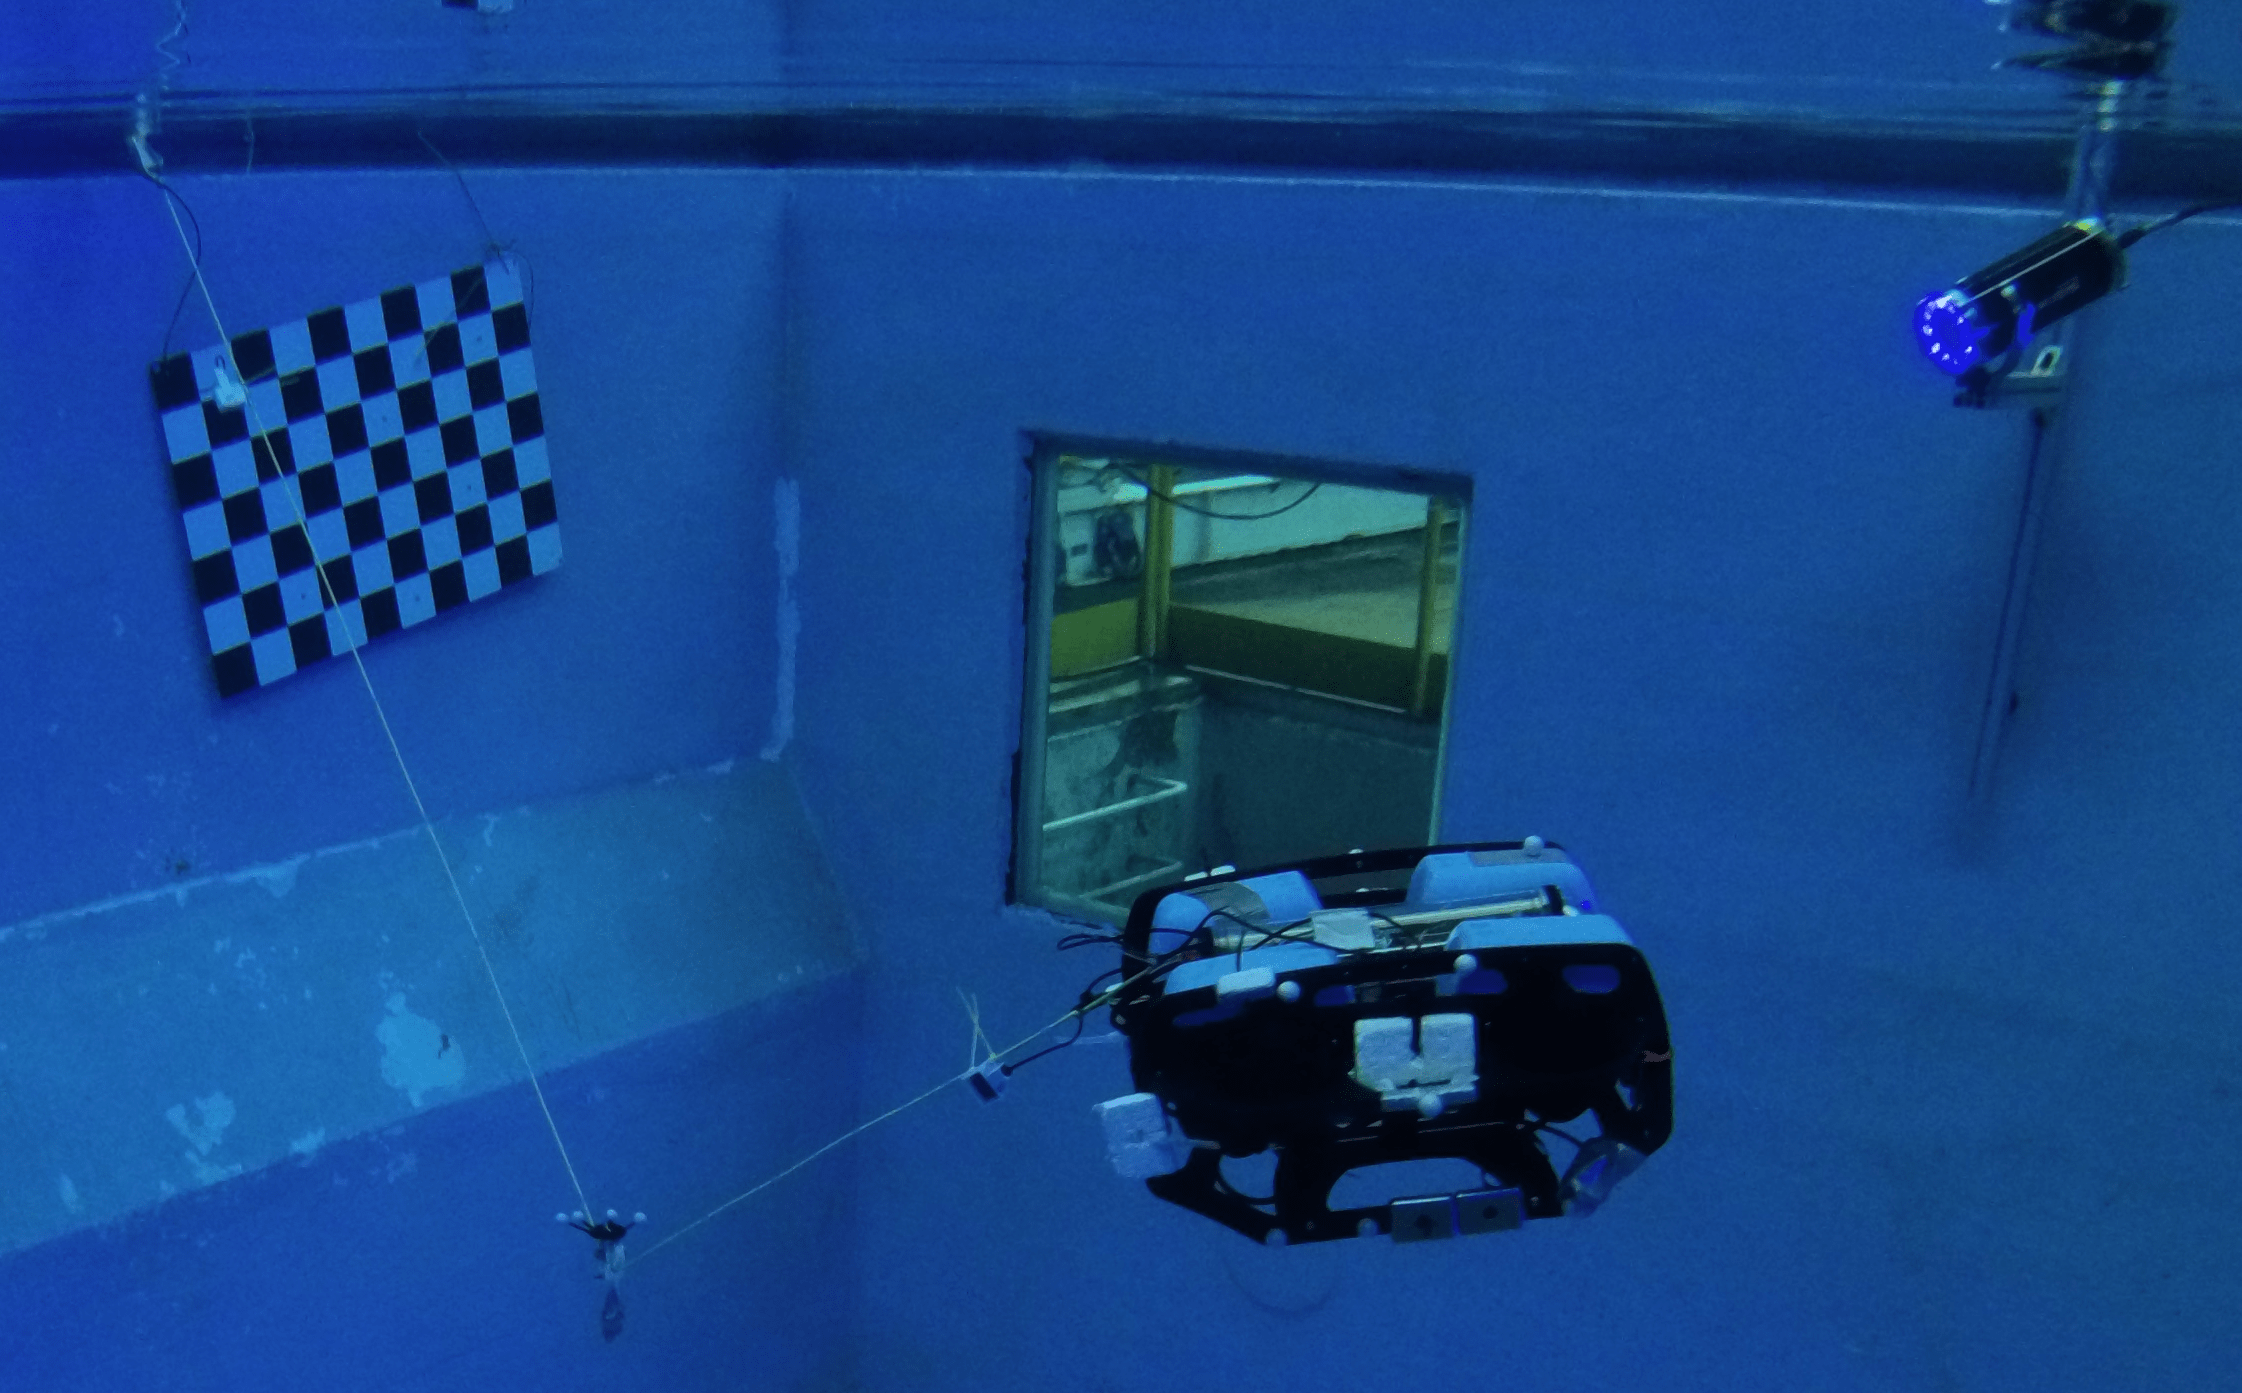
\includegraphics[width=.75\textwidth]{Figures/Cable/Expe/cv_setup.png}};

    % IMUs
    \coordinate (IMU1) at ($(Ppic) + (-2.8,1.)$);
    \draw[orange, thick] (IMU1) node[above=0.35cm, yshift=0.cm] {IMU~1} circle (0.25cm);
    \coordinate (IMU2) at ($(Ppic) + (-0.4,-1.2)$);
    \draw[magenta, thick] (IMU2) node[below=0.35cm, xshift=-0.2cm, align=center] {IMU~2} circle (0.25cm);

    % Attachment points
    \coordinate (O) at ($(Ppic) + (-3.05,1.6)$);
    \draw[white, thick, fill=white] (O) node[above=0.1cm] {$\mathbf{O}$} circle (1pt);
    \coordinate (R) at ($(Ppic) + (0.2,-0.8)$);
    \draw[white, thick, fill=white] (R) node[below=0.1cm] {$\mathbf{R}$} circle (1pt);

    % Label anchors
    \coordinate (Q) at ($(Ppic) + (3.2,1.3)$);
    \coordinate (M1) at ($(Ppic) + (-2.3,0)$);
    \coordinate (M2) at ($(Ppic) + (-1.5,-1.6)$);
    \coordinate (M3) at ($(Ppic) + (1.3,-0.45)$);
    \coordinate (Rob) at ($(Ppic) + (1.5,-1)$);
    \coordinate (B) at ($(Ppic) + (-1.5,-1.9)$);

    % Labels
    \def\labelspacing{0.8}
    \coordinate (L1) at ($(Ppic) + (4,+1.5*\labelspacing)$);
    \coordinate (L2) at ($(L1) + (0,-\labelspacing)$);
    \coordinate (L3) at ($(L2) + (0,-\labelspacing)$);
    \coordinate (L4) at ($(L3) + (0,-\labelspacing)$);
    \node (l1) at (L1) [right] {Mocap camera};
    \node (l2) at (L2) [right, align=left] {Reflective \\ markers};
    \node (l3) at (L3) [right] {BlueROV2};
    % \node (l4) at (L4) [right] {Sliding ballast};

    \path let \p{l1}=(l1.west) in coordinate (l1m) at ({\x{l1} - 0.5cm}, \y{l1});
    \draw[double arrow=2pt colored by white and black] (l1.west) -- (l1m) -- (Q);

    \path let \p{l2}=(l2.west) in coordinate (l2m) at ({\x{l2} - 4cm}, \y{l2});
    \draw[double arrow=2pt colored by white and black] (l2m) -- (M2);
    \draw[double arrow=2pt colored by white and black] (l2m) -- (M3);
    \draw[double arrow=2pt colored by white and black] (l2.west) -- (l2m) -- (M1);

    \path let \p{l3}=(l3.west) in coordinate (l3m) at ({\x{l3} - 1cm}, \y{l3});
    \draw[double arrow=2pt colored by white and black] (l3.west) -- (l3m) -- (Rob);

    % \path let \p{l4}=(l4.west) in coordinate (l4m) at ({\x{l4} - 1cm}, \y{l4});
    % \node (n) at (B) {};
    % \path let \p{B}=(n) in coordinate (l4mbis) at ({\x{B} + 4cm}, \y{B});
    % \draw[double arrow=2pt colored by white and black] (l4.west) -- (l4m) -- (l4mbis) -- (B);

    \draw[yellow, thick] ($(B) + (-0.1,0.1)$) node[left=0.7cm, align=right] {Sliding \\ ballast} circle (0.35cm);

\end{tikzpicture}